\documentclass[a4paper,11pt]{article}
\usepackage{latexsym,amssymb,enumerate,amsmath,epsfig,amsthm}
\usepackage[margin=1in]{geometry}
\usepackage{setspace,color}
\usepackage{graphics}
\usepackage{graphicx}
\usepackage[center, font=footnotesize]{caption}
\usepackage{float}

%\newcommand{\x}{\mathbf{x}}
%\newcommand{\y}{\mathbf{y}}
%\newcommand{\bv}{\mathbf{v}}
%\newcommand{\n}{\mathbf{n}}
%\newcommand{\colored}[1]{\textcolor{red}{#1}}
%\newtheorem{thm}{Theorem}[section]
%\newtheorem{prop}{Proposition}[section]
%\newtheorem{obser}{Observation}[section]
%\newtheorem{corollary}{Corollary}[section]

%\doublespacing
\setlength{\parskip}{1em}

\title{High Resolution Image Construction using Gradient Profile Prior}
\author{
Wilbert Caine\thanks{SID: {\bf 20584260}, Email: {\bf wcaine@connect.ust.hk}}
}

\begin{document}
\thispagestyle{plain}
\maketitle

%\begin{center}
%{\em Supervised by: } Dr. A-B-C 
%\end{center}
%\vspace{0.5cm}

\begin{abstract}
We employed the information in the gradient profile prior to construct high resolution images form the corresponding low resolution images. The reconstructed images are sharp while artifacts are minimal. A sharpness enhancement function can also be introduced to enhance the sharpness of the image. For noisy images, we adopt the non local means algorithm to remove the noise and reuse the noise to recover denoising loss. Some reconstructed high resolution results are attached as example.
\end{abstract}


\section{Introduction}

Image resolution refers to the ability of a sensor to differentiate between two objects or pixels that are relatively close to each other. Compared to low-resolution images (LR), high-resolution (HR) images are often desirable especially in fields such as computer vision, video surveillance, medical imaging, etc. Despite the vast advancement in hardware technology, image resolution enhancement techniques are still significant in many applications. For example, digital surveillance products usually sacrifice not only frame rate but also resolution to ensure the long-term usability of the devices \cite{in16}. The purpose of super-resolution (SR) is to generate a HR image out of the LR image. In general, there are three different approaches, which are interpolation based methods, reconstruction based methods, and learning based methods, with their own advantages and disadvantages in the application \cite{sr11}. Overall, many researches have been done on how to apply the prior or constraint of the HR images.

To solve this issue, the proposed model uses the spatial layouts of natural images gradient to reconstruct the HR image. In this project, the spatial layout of image gradient is described by gradient profile \cite{sr11}. The gradient profile is expressed by an increasing sequence of gradient magnitudes of the pixels crossed by the 1-D path along the magnitude direction passing through the edge pixel. By enforcing both reconstruction constraint and the gradient field constraint, the HR images would be sharp with minimal artifacts along the edges. In this report, we show that the gradient profile prior could be used to enhance the sharpness and control the amount of artifacts in the image. The report is organized as follows. In Section \ref{sec:Gradient Profile Prior}, we study the properties found in the gradient profile prior of natural images which we expect to recover in the HR image given the LR image. In Section \ref{sec:Gradient Profile Prior for Image Super-Resolution}, we present the SR image generation model using the gradient profile prior. Lastly, in Section \ref{sec:Gradient Profile Prior for Image Enhancement}, we discuss how to further enhance the sharpness of an image and one possible approach to produce the HR image of a noisy LR image without the noise being enhanced.

\section{Gradient Profile Prior}
\label{sec:Gradient Profile Prior}

We define the image gradient as $\nabla I = (\partial_x I, \partial_y I) = \sqrt{(\partial_x I)^2 + (\partial_y I)^2} \cdot \vec{N} = m \cdot \vec{N} $ where $m$ is the gradient magnitude and $\vec{N}$ is the gradient unit vector. To obtain the numerical derivatives, we adopts the central difference for both $\partial_x I$ and $\partial_y I$. Then, we denote an edge pixel as the local maximum along a gradient direction of a pixel in the gradient field. In other words, we can trace the path along the gradient direction of an edge pixel until the gradient magnitude stops decreasing. The path from an edge pixel along the gradient direction is called gradient profile. In implementation, piecewise linear interpolation is applied to estimate the gradient of the pixel when one of the spatial coordinates is non-integer (i.e. the gradient magnitude will be compared to the current gradient magnitude only when at least one of the spatial coordinates is an integer). The gradient magnitude and coordinate of the encountered pixels are recorded for further usage.

\begin{figure}[H]
	\centering
	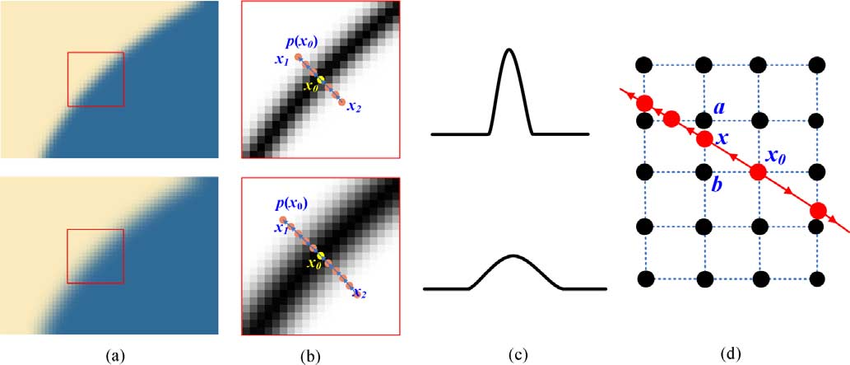
\includegraphics[width=0.8\textwidth]{Gradient-profile-a-Two-edges-with-different-sharpness-b-Gradient-maps-normalized.png}
	\caption{(a) two images with different sharpness where the top image is sharper than the bottom image. (b) inverted and normalized gradient magnitude for the corresponding region of the image in (a) and the gradient profile $p(x_0)$ is the path which starts from the edge pixel $x_0$ along the gradient direction and stops at $x_1$ and $x_2$ where the gradient magnitude no longer decrease. (c) graph of gradient magnitude along the path $p(x_0)$ from  $x_1$ to $x_2$. Note that sharp edge results in shorter gradient profile and more significant jump of gradient magnitude along the gradient profile. (d) encountered pixels are marked by red dots. As an example, the gradient magnitude at $x$ is interpolated from $a$ and $b$ and the gradient magnitude between $x_0$ and $x$ will be disregarded.}
	\label{fig:gp}
\end{figure}

To investigate the gradient profile in natural images, we describe the distribution of gradient profiles as
\begin{equation}
	g(x; \sigma, \lambda) = \frac{\lambda \alpha (\lambda)}{2 \sigma \Gamma(\frac{1}{\lambda})} e^{-[\alpha (\lambda)\lvert \frac{x}{\sigma} \rvert]^\lambda}
\end{equation}
with $\Gamma(\cdot)$ is gamma function and $\alpha (\lambda) = \sqrt{\frac{\Gamma(\frac{3}{\lambda})}{\Gamma(\frac{1}{\lambda})}}$. The shape parameter($\lambda$) controls the distribution shape of the gradient profile. The optimal shape parameter is obtained by varying the value of $\lambda$ on sampled natural images as shown in Figure \ref{fig:shapep} using Kullback-Leibler (KL) divergence as the fitting error. As a result of the findings from \cite{sr11}, the shape parameter is set to 1.6 which is the optimal prior for natural images that minimize the error as observed in Figure \ref{fig:shapep}. It is also shown in Figure \ref{fig:shapep} that shape parameter is resolution independent in natural images. Although bicubic interpolation may influence the shape parameter, it is found that the optimal $\lambda$ is 1.63 for images with up-sampling factor of 2. 

\begin{figure}[H]
	\centering
	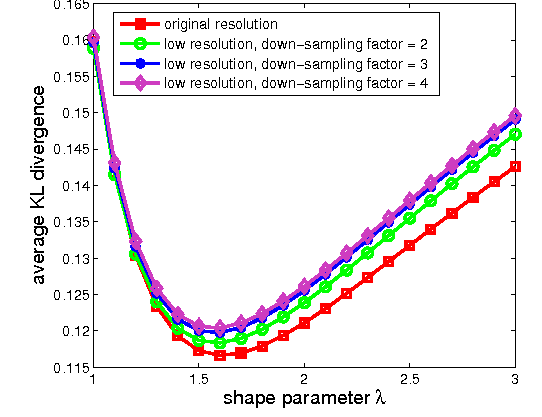
\includegraphics[width=0.4\textwidth]{3-Figure2-1.png}
	\caption{average KL-divergence between the gradient profiles of various shape parameter $\lambda$ and the fitted gradient profiles}
	\label{fig:shapep}
\end{figure}

The gradient profile sharpness of an edge pixel is defined as
\begin{equation}
	\label{eq:sigma}
	\sigma_l(p(x_0)) = \sqrt{\sum_{x \epsilon p(x_0)} m'(x) d^2(x, x_0)}
\end{equation}
where $m'(x) = {m(x) \over \sum_{x \epsilon p(x_0)} m(x)}$ and $d(x,x_0)$ is the distance between $x$ and $x_0$ along the gradient direction $p(x_0)$. Intuitively, sharp gradient profile has low $\sigma$ value. Initially, the equation (\ref{eq:sigma}) is used to find the sharpness of the up-sampled image from the LR image. The sharpness $\sigma_h$ in the HR image, which is to be constructed, could be estimated from the sharpness $\sigma_l$ based on the learning of natural images (shown in Figure \ref{fig:es}). Finally, the expected sharpness of the HR image is computed using hardcoded data from the learning.

\begin{figure}[H]
	\centering
	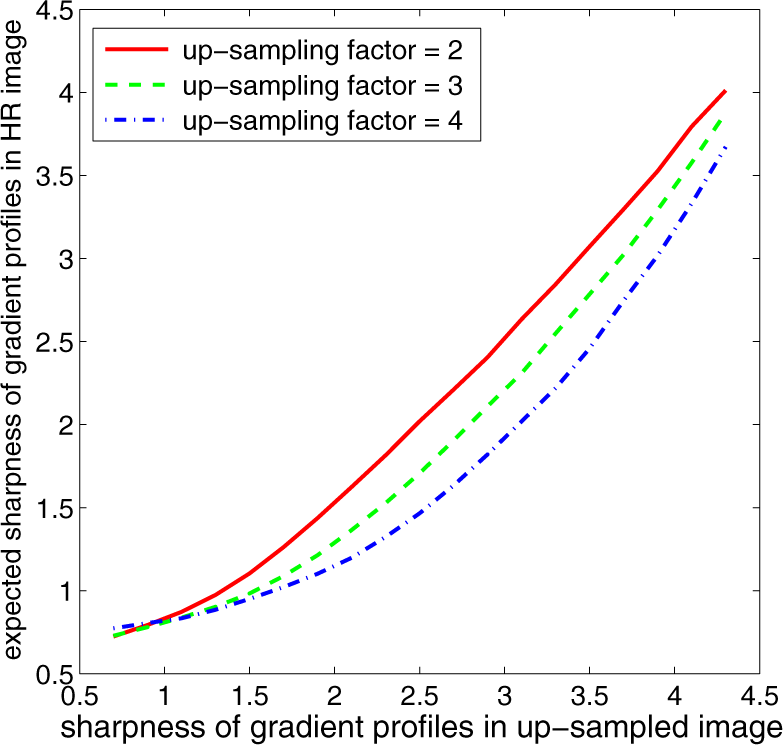
\includegraphics[width=0.4\textwidth]{Expected-sharpness-of-the-gradient-profiles-in-HR-image-with-respect-to-sharpness-of-the.png}
	\caption{relationship between the sharpness of gradient profiles in up-sampled images and the sharpness of gradient profiles in the actual HR image.}
	\label{fig:es}
\end{figure}

\section{Gradient Profile Prior for Image Super-Resolution}
\label{sec:Gradient Profile Prior for Image Super-Resolution}

In this project, the HR gradient field is approximated from the LR gradient field using the gradient profile prior. We denote gradient profile as $p_l$ for up-sampled LR image $I_l^u$ and $p_h$ for the HR image $I_h$. Firstly, we compute the ratio between the gradient profiles, i.e.
\begin{equation}
	\label{eq:transformr}
	r(d(x, x_0)) = \frac{g(d(x, x_0); \sigma_h, \lambda_h)}{g(d(x, x_0); \sigma_l, \lambda_l)}
\end{equation}
where $\lambda_h=1.63$, $\lambda_l=1.6$, and $\sigma_h$ is estimated from $\sigma_L$ using the pre-computed data from the learning result in section \ref{sec:Gradient Profile Prior}. Thus, we estimate $p_h$ by multiplying $p_l$ by the transform ratio in (\ref{eq:transformr}), i.e. the transformed HR gradient field is denoted by
\begin{equation}
	\label{eq:transformgrad}
	\nabla I_h^T(x) = r(d(x, x_0)) \cdot \nabla I_l^u(x)
\end{equation}
for every pixel $x$ in the image. Multiplying the transform ratio results in increased gradient magnitude of the pixels near an edge pixels or decreased otherwise. In Figure \ref{fig:picture1}, the gradient magnitude within the distance of $d_0$ will be increased and otherwise will be decreased. Through this process, the gradient profile sharpness is enhanced while the spatial scattering becomes smaller which is illustrated in Figure \ref{fig:gp} (c).

\begin{figure}[H]
	\centering
	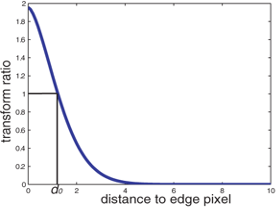
\includegraphics[width=0.4\textwidth]{Picture1.png}
	\caption{An example of the graph of transform with parameters value of $\lambda_h=1.6$, $\sigma_h=1$, $\lambda_l=1.6$, and $\sigma_l=2$. The transform ratio within $d_0$ is larger than 1 while the transform ratio outside $d_0$ is smaller than 1. As a result, the gradient magnitude will be increased within $d_0$ and decreased outside $d_0$.}
	\label{fig:picture1}
\end{figure}

In addition to the image domain constraint, the transformed gradient field in (\ref{eq:transformgrad}) is also used as the gradient domain constraint when reconstructing the HR image. Given a LR image $I_l$, we minimize the following energy to reconstruct the HR image $I_h$
\begin{equation}
	\label{eq:energy1}
	E(I_h | I_l, \nabla I_h^T) = E_i(I_h | I_l) + \beta E_g(\nabla I_h, \nabla I_h^T) 
\end{equation}
where $E_i$ is the constraint in the image domain denoted by
\begin{equation}
	\label{eq:energyi}
	E_i(I_h | I_l) = \lvert (I_h \ast G) \downarrow - I_l \rvert^2
\end{equation}
,with convolution operator $\ast$, down-sampling operator $\downarrow$, and gaussian filter $G$ with standard deviation 0.8 for up-sampling factor of 2, while $E_g$ is the constraint in the gradient domain denoted by
\begin{equation}
	\label{eq:energyg}
	E_g(\nabla I_h, \nabla I_h^T) = \lvert \nabla I_h - \nabla I_h^T \rvert^2
\end{equation}
By applying the constraint in the gradient domain, the gradient profile in reconstructed HR image $I_h$ is encouraged to have the desired statistics of those in natural HR images.

In practice, we use the following iterative scheme to minimize (\ref{eq:energy1})
\begin{equation}
	I_h^{t+1} = I_h^t - \tau \cdot \frac{\partial E(I_h)}{\partial I_h}
\end{equation}
where
\begin{equation}
	\frac{\partial E(I_h)}{\partial I_h} = ((I_h \ast G) \downarrow - I_l) \uparrow \ast G - \beta \cdot (div(\nabla I_h) - div(\nabla I_h^T))
\end{equation}
 with $div(\nabla I_h) = \frac{\partial^2 I_h}{\partial x^2} + \frac{\partial^2 I_h}{\partial y^2}$ and step function $\tau =0.2$ by default.

Parameter $\beta$ is introduced to the model to balance the image domain constraint and gradient domain constraint. Large value of $\beta$ corresponds to placing more importance on the gradient domain constraint, which results in sharp edge with little artifacts. Conversely, small value $\beta$ places higher emphasis on the image domain constraint. Smaller value of $\beta$ leads to better image contrast, however, ringing or jaggy artifacts may be introduced at the edges. Figure \ref{fig:beta2} better illustrates the difference of high and low values of $\beta$.

\begin{figure}[H]
	\centering
	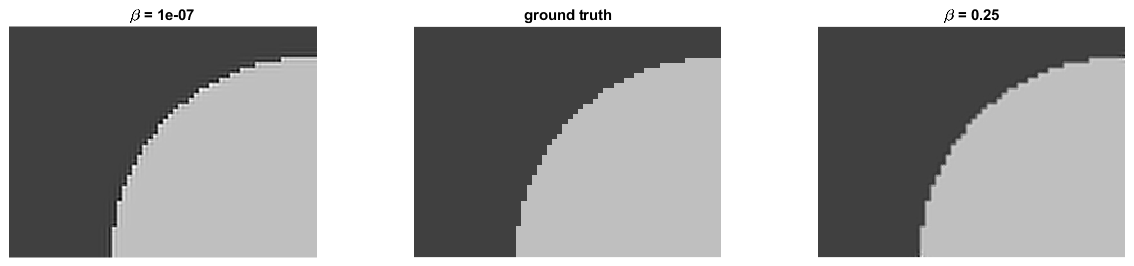
\includegraphics[width=1\textwidth]{large small beta.png}
	\caption{HR image reconstruction with small and large value of parameter $\beta$. Setting small value of $\beta$ will produce HR image with ringing and jaggy artifacts. On the other hand, the artifacts are less visible when $\beta$ is larger.}
	\label{fig:beta2}
\end{figure}
 
After the HR image is generated, we assess the performance of the model by comparing the structural similarity index measure (SSIM) between the SR image and the original image. The SSIM value is based on three different measurement, such as luminance ($l$), contrast ($c$), and structure ($s$), i.e.
\begin{gather*}
	l(x,y) = \frac{2 \mu_x \mu_y + c_1}{\mu_x^2 + \mu_y^2 + c_1}\\
	c(x,y) = \frac{2 \sigma_x \sigma_y + c_2}{\sigma_x^2 + \sigma_y^2 + c_2}\\
	s(x,y) = \frac{2 \sigma_xy + c_2}{\sigma_x \sigma_y + c_2}\\
	SSIM(x,y) = [l(x,y)^\alpha \cdot c(x,y)^\beta \cdot s(x,y)^\gamma]
\end{gather*}
where $c_3 = \frac{c_1}{2}$, $c_1=(k_1L)^2$, and $c_2=(k_2L)^2$ with $k_1=0.01$, $k_2=0.03$, and $L=2^{\#bits\ per\ pixel}-1$ by default. In practice, we let $\alpha = \beta = \gamma = 1$. The resultant of SSIM index is a value between 0 and 1 where a value of 0 indicates no structural similarity and a value of 1 is only obtained when two identical images are compared. Therefore, we can use SSIM value as a measurement to determine the value of $\beta$ that produces the best HR result. For the series of $\beta$ values in Figure \ref{fig:beta}, we found that $\beta = 0.05$ produces the best result in terms of SSIM by experiment.

\begin{figure}[H]
	\centering
	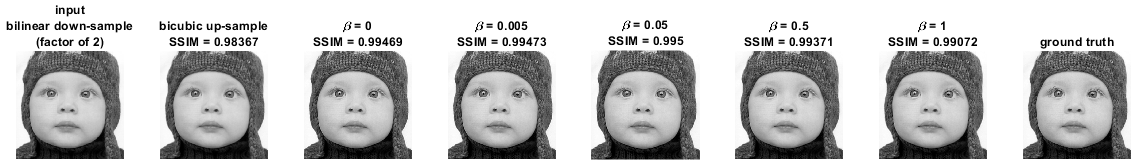
\includegraphics[width=1\textwidth]{beta.png}
	\caption{Effect of changing the value of the parameter $\beta$ towards the SSIM between the reconstructed HR image and the ground truth. We set $\beta = 0.05$, by default, in the implementation. In experiment, the HR images are sharp and clear enough after 25 iterations (default number of iterations in the implementation).}
	\label{fig:beta}
\end{figure}

\section{Gradient Profile Prior for Image Enhancement}
\label{sec:Gradient Profile Prior for Image Enhancement}

\subsection{Sharpness Enhancement Function}

HR images are expected to have sharp edges to be considered as sharp image. This sharpness is identified by the $\sigma_h$ value in the model. In addition to the gradient field transformation, the sharpness enhancement function could be applied to further enhance the sharpness of blurry edges. The sharpness enhancement function can be expressed as
\begin{equation}
	F(\sigma_h) = (1-e^{-\mu\sigma_h})\sigma_h
\end{equation}
which is continuous and results in smaller $\sigma_h$ values. As $\mu > 0$ is chosen to be closer to 0, the edge sharpness will be further enhanced. When $\mu = \infty$, the model will have no sharpness enhancement and corresponds to the original model.

\begin{figure}[H]
	\centering
	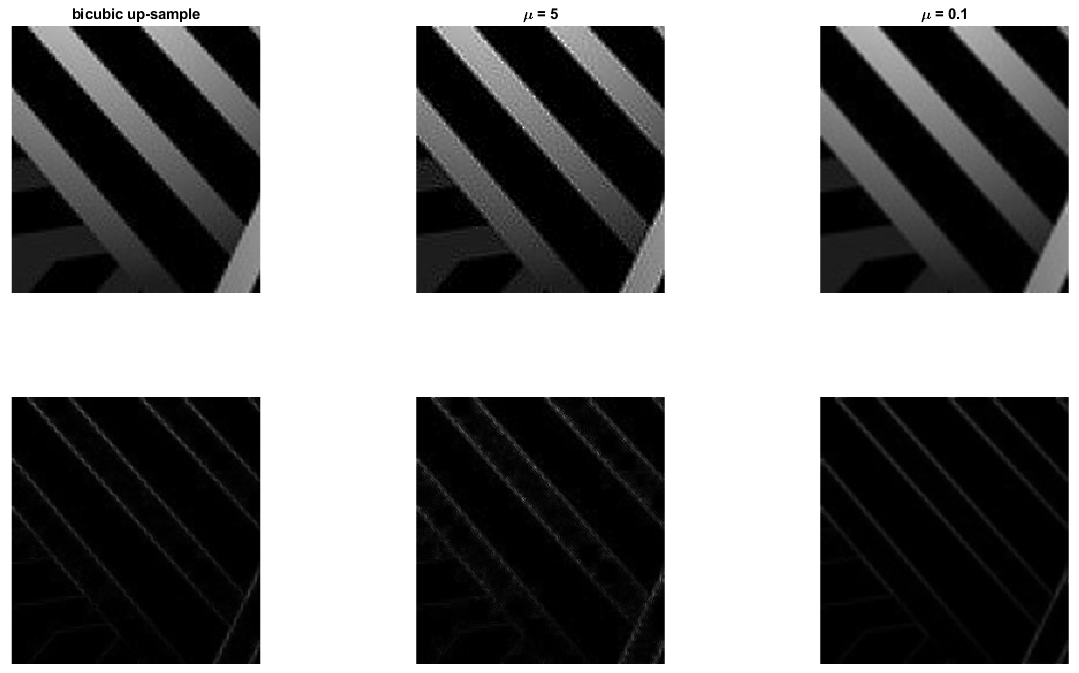
\includegraphics[width=1\textwidth]{mu variation.png}
	\caption{Image enhancement using the sharpness enhancement function: the reconstructed HR images (top) and inverted gradient magnitude map (bottom). After sharpness enhancement, the length of the gradient profile becomes shorter than the gradient profile prior before applying the function. This is represented by the thinner white lines in the bottom right image. The difference in the gradient maps is similar to our initial observation in Figure \ref{fig:gp} (b).}
	\label{fig:mu}
\end{figure}


\subsection{Noisy Image Super-Resolution}

One may expect that the model could be sensitive to noise such that the noise would be sharpened as well. The SR model using the gradient profile prior is incapable of differing between edge and noise in the image. In other words, the model will treat the noise in the same way as the edge, i.e. enhanced. As an implication, the noise might appear as local maximum in the gradient domain and, in turns, create unexpected gradient profiles. One straightforward solution is to firstly extract the noise layer through a denosing method before applying the HR reconstruction algorithm. This process would remove the unexpected gradient profiles in the image. Secondly, the noise layer is then upsampled and reapplied to the HR image constructed previously. In Figure \ref{fig:sden}, the LR image is denoised with the non-local means algorithm \cite{nlm05} to obtain a more pleasant result to our eye (bottom right) compared to the original result (top right). The worsened HR of noisy LR is also reflected by the SSIM index where both the up-sampled image and the HR of denoised LR with re-added noise have higher SSIM values when compared to the original image. This is because not only the edge but also the noise in the noisy LR is enhanced by the model, whereas the noise in the HR of denoised LR have been extracted beforehand thus not enhanced. 

\begin{figure}[H]
	\centering
	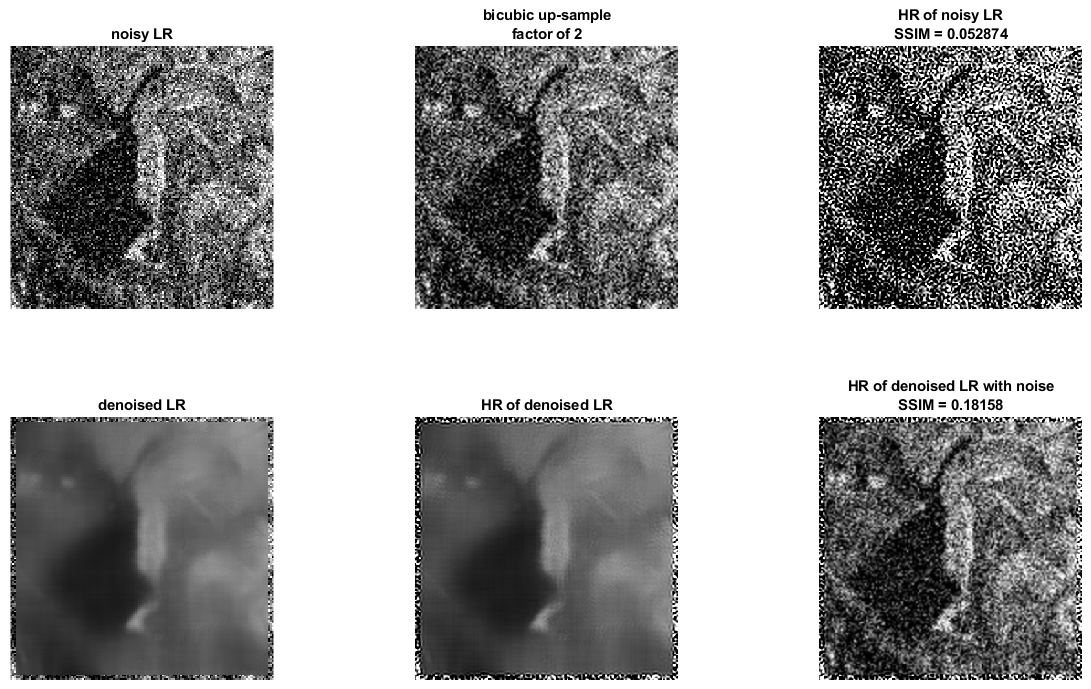
\includegraphics[width=1\textwidth]{simple denoise.png}
	\caption{(top) HR image reconstruction from the noisy LR image. (bottom) HR image is reconstructed by adding back the up-sampled noise layer to the HR image generated from the denoised LR image}
	\label{fig:sden}
\end{figure}

\section{Conclusion}

In this project, we have utilized natural image prior called the gradient profile prior. The gradient field of up-sampled LR image is transformed using the gradient profile prior and, in addition to the image domain constraint, the transformed gradient field is applied as a constraint in the gradient domain. The model produce HR image with enhanced sharpness and suppressed ringing or jaggy artifacts while the sharpness distribution is enforced to fit the distribution from learned natural images. The examples of the resulting image in the project is verified with the SSIM value between the HR image and the ground truth. The sharpness enhancement function could also be incorporated into the model to further enhance the sharpness of the image. For noisy images, one possible approach is to apply any denoising technique to remove the noise and re-add the noise back after HR image is reconstructed from the denoised image. In the future, one may consider other image reconstruction applications using the gradient profile prior.

\begin{thebibliography}{10}

\bibitem{in16} {\sc Yue, Linwei \& Shen, Huanfeng \& Li, Jie \& Yuan, Qiangqiang \& Zhang, Hongyan \& Zhang, Liangpei.} (2016). {\em Image super-resolution: The techniques, applications, and future.} Signal Processing. 128. 10.1016/j.sigpro.2016.05.002. 

\bibitem{sr11} {\sc J. Sun, J. Sun, Z. Xu, \& H. Shum}, {\em Gradient Profile Prior and Its Applications in Image Super-Resolution and Enhancement}, in IEEE Transactions on Image Processing, vol. 20, no. 6, pp. 1529-1542, June 2011.

\bibitem{ssim04} {\sc Zhou Wang, A. C. Bovik, H. R. Sheikh, \& E. P. Simoncelli}, {\em Image quality assessment: from error visibility to structural similarity}, in IEEE Transactions on Image Processing, vol. 13, no. 4, pp. 600-612, April 2004.

\bibitem{nlm05} {\sc A. Buades, B. Coll, \& J. -. Morel}, {\em A non-local algorithm for image denoising}, 2005 IEEE Computer Society Conference on Computer Vision and Pattern Recognition (CVPR'05), San Diego, CA, USA, 2005, pp. 60-65 vol. 2.

\end{thebibliography}

\end{document}
